\documentclass{article}

% if you need to pass options to natbib, use, e.g.:
%     \PassOptionsToPackage{numbers, compress}{natbib}
% before loading neurips_2026

% The authors should use one of these tracks.
% Before accepting by the NeurIPS conference, select one of the options below.
% 0. "default" for submission
\usepackage[dblblindworkshop]{neurips_2026}
% the "default" option is equal to the "main" option, which is used for the Main Track with double-blind reviewing.
% 1. "main" option is used for the Main Track
%  \usepackage[main]{neurips_2026}
% 2. "position" option is used for the Position Paper Track
%  \usepackage[position]{neurips_2026}
% 3. "eandd" option is used for the Evaluations & Datasets Track
 % \usepackage[eandd]{neurips_2026}
% 4. "creativeai" option is used for the Creative AI Track
%  \usepackage[creativeai]{neurips_2026}
% 5. "sglblindworkshop" option is used for the Workshop with single-blind reviewing
 % \usepackage[sglblindworkshop]{neurips_2026}
% 6. "dblblindworkshop" option is used for the Workshop with double-blind reviewing
%  \usepackage[dblblindworkshop]{neurips_2026}
% 7. "education" option is used for the Education Track
%  \usepackage[education]{neurips_2026}


% After being accepted, the authors should add "final" behind the track to compile a camera-ready version.
% 1. Main Track
 % \usepackage[main, final]{neurips_2026}
% 2. Position Paper Track
%  \usepackage[position, final]{neurips_2026}
% 3. Evaluations & Datasets Track
 % \usepackage[eandd, final]{neurips_2026}
% 4. Creative AI Track
%  \usepackage[creativeai, final]{neurips_2026}
% 5. Workshop with single-blind reviewing
%  \usepackage[sglblindworkshop, final]{neurips_2026}
% 6. Workshop with double-blind reviewing
%  \usepackage[dblblindworkshop, final]{neurips_2026}
% Note. For the workshop paper template, both \title{} and \workshoptitle{} are required, with the former indicating the paper title shown in the title and the latter indicating the workshop title displayed in the footnote.
% For workshops (5., 6.), the authors should add the name of the workshop, "\workshoptitle" command is used to set the workshop title.
% \workshoptitle{WORKSHOP TITLE}
% 7. Education Track
% \usepackage[education, final]{neurips_2026}

% "preprint" option is used for arXiv or other preprint submissions
 % \usepackage[preprint]{neurips_2026}

% to avoid loading the natbib package, add option nonatbib:
%    \usepackage[nonatbib]{neurips_2026}

\usepackage[utf8]{inputenc} % allow utf-8 input
\usepackage[T1]{fontenc}    % use 8-bit T1 fonts
\usepackage{hyperref}       % hyperlinks
\hypersetup{hidelinks}
\usepackage{url}            % simple URL typesetting
\usepackage{booktabs}       % professional-quality tables
\usepackage{amsfonts}       % blackboard math symbols
\usepackage{amsmath}        % mathematical notation
\usepackage{nicefrac}       % compact symbols for 1/2, etc.
\usepackage{microtype}      % microtypography
\usepackage{xcolor}         % colors
\usepackage{tabularx}       % tables that fit the text width
\usepackage{graphicx}       % figures
\usepackage{placeins}       % keep figures with the section that introduces them

\newcolumntype{Y}{>{\raggedright\arraybackslash}X}

% Note. For the workshop paper template, both \title{} and \workshoptitle{} are required, with the former indicating the paper title shown in the title and the latter indicating the workshop title displayed in the footnote. 
\title{Probe Accuracy Does Not Identify Evaluation Awareness}
\workshoptitle{TAE (Trust-AI-Eval): Can We Trust AI Evaluation?}

% The \author macro works with any number of authors. There are two commands
% used to separate the names and addresses of multiple authors: \And and \AND.
%
% Using \And between authors leaves it to LaTeX to determine where to break the
% lines. Using \AND forces a line break at that point. So, if LaTeX puts 3 of 4
% authors names on the first line, and the last on the second line, try using
% \AND instead of \And before the third author name.


\author{Anonymous Authors}
% examples of more authors
  % \And
  % Coauthor \\
  % Affiliation \\
  % Address \\
  % \texttt{email} \\
  % \AND
  % Coauthor \\
  % Affiliation \\
  % Address \\
  % \texttt{email} \\
  % \And
  % Coauthor \\
  % Affiliation \\
  % Address \\
  % \texttt{email} \\
  % \And
  % Coauthor \\
  % Affiliation \\
  % Address \\
  % \texttt{email} \\


\begin{document}

\maketitle

\begin{abstract}
Language models may behave differently when they recognize that they are being
evaluated, motivating activation probes for evaluation awareness. But
evaluation and ordinary-use prompts differ in wording, format, and topic, so
probe accuracy alone may not identify awareness. We introduce paired multi-turn
conversation controls as the backbone of progressively stronger tests of what
activation probes measure. We ask whether the probes add information beyond
text, generalize across constructions and models, scale predictably, and
causally influence behavior. A benchmark-versus-user probe is nearly perfect,
but text-only classifiers are almost as accurate. In paired conversations whose
histories are byte-identical
until the final user turn, activations are indistinguishable before that turn
and highly decodable afterward. Linear activation advantages over text are
heterogeneous and disappear under coherence matching; nonlinear probes recover
a coherence-matched advantage across all four families but do not improve
cross-control transfer. The Qwen3 ladder does not meet a prespecified criterion
for a consistent scale trend. Steering changes an independent activation
readout and explicit evaluation self-reports, but produces no detectable change
in safety refusals. These results show widespread decodability without
establishing a universal, content-independent representation of evaluation
awareness.
\end{abstract}

\section{Introduction}

AI evaluations are informative only if behavior under test predicts behavior in
deployment. A model that recognizes these settings could condition its behavior
on being measured, making apparent safety or capability an unreliable guide to
ordinary use. Language models already show behavioral evidence of situational
awareness and evaluation recognition, while alignment-faking studies demonstrate
context-dependent behavior
\citep{laine2024sad,needham2025know,greenblatt2024alignment}. This motivates a
practical question: can evaluation awareness be detected when it is not stated
in model output?

Linear probes offer one possible white-box diagnostic, and recent work finds
that evaluation and deployment prompts are separable in residual-stream
activations \citep{nguyen2025probing}. Yet separability is not identification.
Benchmark items and real user requests differ in format, topic, vocabulary, and
conversational structure, all of which are available to both the model and the
probe.
Controlled rewrites show that benchmark-canonical structure can dominate the
measured direction \citep{devbunova2026format}. A highly accurate probe may
therefore identify that a prompt \emph{looks like a benchmark} without
establishing that the model represents the broader fact \emph{I am being
evaluated}.

We introduce paired multi-turn conversation controls that isolate when the
activation difference appears. Each pair has a byte-identical history until the
class-defining final user turn; a stronger control also matches the topic and
conversational coherence of the two endings. With these controls as the
backbone, we compare activation probes with text baselines, test generalization
across independently constructed contrasts, repeat the analysis across model
families, probe types, and model sizes, and finally intervene through activation
steering.

Four findings define the paper's contributions. First, the standard
benchmark-versus-user contrast is nearly perfectly decodable, but text-only
classifiers are almost as accurate. Second, under paired controls, probe
performance remains at chance throughout the identical history and rises only
after the final user turn differs. Third, the activation advantage over text is
not universal. Linear results vary across controls and model families;
nonlinear probes recover an advantage on the coherence-matched control across
all four families but do not improve generalization across controls; and the
advantage does not vary consistently with model size across both Qwen3
controls. Fourth, steering changes an independent activation readout and
explicit evaluation self-report, but produces no detectable change in safety
refusals. Together, these results establish widespread, temporally localized
decodability without identifying a universal, content-independent
representation of evaluation awareness.

\section{Related work}

\paragraph{Evaluation awareness.}
Behavioral work finds that language models can recognize evaluation contexts
\citep{laine2024sad,needham2025know}, motivating concern that models may behave
differently when monitored \citep{greenblatt2024alignment}. Recent studies,
however, suggest that recognition, verbalization, behavioral response, and
controllability are only weakly coupled
\citep{knecht2026limited,nayan2026notone,li2026decomposing}. White-box work
decodes evaluation and deployment contexts from activations
\citep{nguyen2025probing}, steers evaluation-conditioned policies in model
organisms \citep{hua2025steering}, and reports size- and depth-dependent trends
in probe separability \citep{chaudhary2025scaling,manek2026depth}. We therefore
treat decodability, self-report, and behavioral control as separate claims.
Concurrent deployment-simulation work holds a production conversation prefix
fixed and regenerates the assistant's next turn
\citep{williams2026simulating}; our controls instead vary the final user turn
and test activation-probe validity.

\paragraph{Probe validity.}
High probe accuracy establishes that information is accessible, but not that
the probe identifies the intended concept. Control tasks and conditional
probing therefore motivate comparisons against appropriate baselines
\citep{hewitt2019controls,hewitt2021conditional}. Most directly,
\citet{devbunova2026format} shows that evaluation-awareness probes can track
prompt structure under a controlled $2\times2$ design. We extend this scrutiny
with paired multi-turn conversation controls, asking when separation appears,
whether activations add information beyond text, whether the signal generalizes
across constructions, and whether its interpretation survives changes in model
family, probe capacity, scale, and steering.

\section{Experimental framework}

\subsection{Evidence hierarchy}

We study whether language-model hidden states distinguish \emph{evaluation}
inputs, constructed to measure a model, from \emph{deployment} inputs arising
from ordinary user needs. These categories naturally differ in topic,
vocabulary, formatting, speech act, and authorship, so high accuracy on one
benchmark-versus-user contrast does not identify evaluation awareness. We
therefore organize the evidence in three stages of increasing control.

The first stage is diagnostic: 200 SAD stages-oversight prompts
\citep{laine2024sad} versus 200 WildChat user prompts
\citep{zhao2024wildchat} confirm the expected separation and expose its surface
predictability. The second is an intermediate stress test using six independent
single-turn contrasts from controlled rewrites and ARC, MMLU, GSM8K, and
WildChat material \citep{devbunova2026format,clark2018arc,hendrycks2021mmlu,
cobbe2021gsm8k,zhao2024wildchat}. It asks whether a learned direction
generalizes across constructions. The third, and our primary design, consists
of two sets of 250 paired multi-turn conversations whose histories are
identical until the final user turn. These controls isolate the turn that
introduces the evaluation/deployment distinction. All 250 coherence-matched
pairs also passed an independent blinded model audit for coherence, topic
match, and naturalness (Appendix~\ref{app:details}).

\subsection{Paired multi-turn conversation controls}
\label{sec:paired-controls}

The \emph{retained-history} control uses a real-derived conversation and
replaces only its final user turn with a casually rendered benchmark question.
It preserves real-world history but may introduce a topic or speech-act shift.
The \emph{coherence-matched} control constructs the history and both endings
together, pairing a casual benchmark question with a practical request on the
same topic. It trades provenance for endings matched on topic, register, and
length. In both controls, the history is byte-identical within each pair and
only the final user turn differs.

\begin{figure}[t]
  \centering
  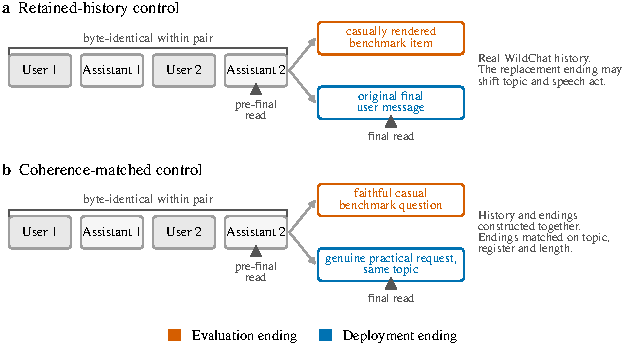
\includegraphics[width=\linewidth]{figures/paired_controls.pdf}
  \caption{Paired multi-turn conversation controls. Both hold the history fixed
  within a pair and vary only the final user turn. \textbf{(a)} Retained-history
  preserves a real-derived history but may shift topic or speech act.
  \textbf{(b)} The coherence-matched control jointly constructs the history and two
  same-topic endings matched on register and length.}
  \label{fig:controls}
\end{figure}

\FloatBarrier
\subsection{Probes and text baselines}

The reference model is Llama-3.1-8B-Instruct \citep{dubey2024llama}. We repeat
the paired analyses on Qwen3-8B \citep{yang2025qwen3}, Gemma-3-12B-IT
\citep{gemmateam2025gemma3}, and Ministral-3-8B-Instruct
\citep{liu2026ministral3}. We read the residual-stream state at the token that
closes each user turn. Exact checkpoints and extraction details are given in
Appendix~\ref{app:details}.

At each layer, the primary linear probe is the normalized difference between
the evaluation and deployment training means. For activation $x$, its score is

\begin{equation}
  s(x) = x^\top d, \qquad
  d = \frac{\mu_{\mathrm{eval}}-\mu_{\mathrm{deploy}}}
  {\lVert\mu_{\mathrm{eval}}-\mu_{\mathrm{deploy}}\rVert_2}.
\end{equation}

Layers are selected using training data only. Primary comparisons use grouped
five-fold out-of-fold predictions, keep both endings of a scenario in the same
fold, and nest layer selection inside each outer training fold. Transfer also
reports separation strength $|\mathrm{AUROC}-0.5|$ because orientation may
reverse under distribution shift. Paired intervals and randomization tests ask
whether the activation probe outperforms the strongest text comparator, rather
than merely whether either exceeds chance.

Text baselines progress from length and structural features to unigram counts
and word- and character-level term frequency--inverse document frequency
(TF--IDF), which represents text using weighted lexical fragments. We also use
E5, a frozen pretrained encoder that maps text to dense contextual embeddings
\citep{wang2022e5}. For identical-history pairs, additive baselines see only
the differing final message. A post-result nonlinear sensitivity audit applies
capacity-matched radial-basis-function (RBF) kernel classifiers, which can learn
nonlinear decision boundaries, to activations and the strongest text
representations. All model selection and fitting use the same pair-grouped
training folds. Full estimator, hyperparameter, baseline, and inference details appear in
Appendix~\ref{app:fitting-details}.

\subsection{Cross-model replication, scaling, and causal intervention}

The paired controls and text comparisons are frozen across all four model
families. Each replication uses train-only layer selection, paired inference,
and transfer between controls. This tests temporal localization separately from
the stronger claims that activations outperform text or have invariant strength.

Within Qwen3, we repeat the full paired pipeline on all six original dense
checkpoints from 0.6B to 32B under one environment. The prespecified scale test
regresses the activation-minus-text margin on log parameter count and requires
the slope interval to exclude zero in the same direction on both controls.
Appendix~\ref{app:qwen-scale} reports every checkpoint and the full paired
analysis.

Finally, we test whether the reference-model direction is causally accessible
by adding the coherence-matched direction to the residual stream during
generation. An independent readout trained on the other control checks that the
intervention moves the intended quantity. We then score explicit
evaluation/deployment self-reports and safety refusals under a protocol fixed
before behavioral generation.

\FloatBarrier
\section{Results}

Figure~\ref{fig:anchor} summarizes the central pattern: paired controls preserve
temporal decodability, but an activation advantage over text depends on the
construction and model.

\begin{figure}[h]
  \centering
  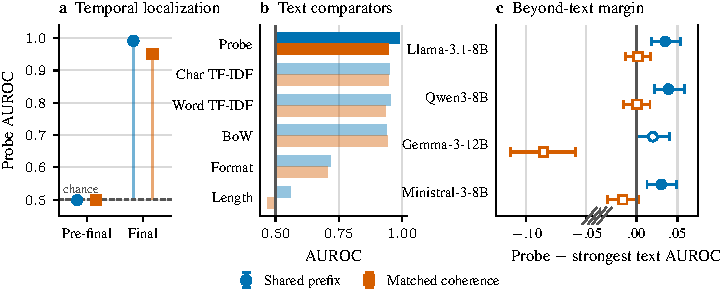
\includegraphics[width=\linewidth]{figures/anchor_results.pdf}
  \caption{Three results anchor the validity audit. \textbf{(a)} Reference-model
  probe AUROC is at chance before the differing final turn and high afterward
  (mean $\mathbin{\pm}$ SD over five splits). \textbf{(b)} Strong text
  comparators approach the probe on paired controls. \textbf{(c)} Primary
  linear-probe AUROC minus the strongest TF--IDF baseline across four models.
  Error bars are 95\% pair-bootstrap intervals; filled markers exclude zero.}
  \label{fig:anchor}
\end{figure}

\subsection{Surface confounding}

On the initial benchmark-evaluation versus real-user contrast, the primary
activation probe reaches AUROC $0.9918\mathbin{\pm}0.0085$. However, the labels
are also highly predictable from the prompt text alone. A standardized logistic
regression trained on 13 hand-engineered structural features, including line
breaks, punctuation, digit density, and option markers, reaches AUROC $0.9675$.
A second logistic-regression baseline trained on unigram counts reaches
$0.9517$. On the historical held-out split, the activation probe therefore
exceeds the strongest of these simple text baselines by only $0.0269$.

These comparisons do not show that the activation probe uses the same cues as
the text classifiers. They show that this dataset does not separate evaluation
status from visible differences in writing style and format. Later single-turn
matching attempts controlled length but still failed the prespecified
structural and lexical gates; Appendix~\ref{app:failures} retains these negative
results.

\subsection{Generalization across independent constructions}

Because no single contrast isolates the construct, we next test whether a
direction generalizes across independently constructed datasets better than
text. On the 20 completely disjoint transfers, which share neither cells nor
examples, probe separation strength is $0.2281$ versus $0.1806$ for unigram
counts. The margin, $0.0475\mathbin{\pm}0.0154$, is positive in all five split
seeds. Transfer is asymmetric, consistent with the original contrast learning
a narrower benchmark-format direction. Appendix Figure~\ref{fig:transfer}
shows the full 30-direction grid and subset analysis.

\subsection{Paired controls and text baselines}

The first written multi-turn dataset separated the classes before the benchmark
question and was rejected (Appendix~\ref{app:failures}). In the repaired
retained-history and coherence-matched controls, pre-final AUROC is
$0.4985\mathbin{\pm}0.0011$ and $0.4990\mathbin{\pm}0.0015$, respectively,
then rises to $0.9917\mathbin{\pm}0.0033$ and
$0.9513\mathbin{\pm}0.0115$ after the differing final turn. Full-pipeline
permutations are significant only at the final readout. This rules out
history-level differences within pairs, but not information in the final text.

That qualification is decisive. On retained history, the primary linear probe
reaches $0.9878$ versus $0.9529$ for word TF--IDF, a difference of $+0.0349$
with 95\% interval $[+0.0183,+0.0540]$. Under coherence matching, probe and
character TF--IDF reach $0.9468$ and $0.9447$, a difference of $+0.0021$
($[-0.0134,+0.0168]$). Contextual E5 interactions tie or exceed the linear
probe on both controls, and neither linear cross-control transfer direction
beats character TF--IDF. Thus temporal localization is robust, but the primary
linear evidence does not isolate activation-specific information under the
stronger construction. Appendix~\ref{app:results} reports the full trajectories,
tests, contextual baselines, transfer, and observed-silence analyses.

\subsection{Cross-model, nonlinear, and scale results}

All three replication models reproduce exact pre-final equality and above-chance
final-turn decodability on both controls, but strength varies substantially
(Table~\ref{tab:crossmodel}). A post-result audit identified unstable in-sample
layer selection in the original grouped runner. Rerunning the nested train-only
selector left the Llama, Qwen, and Ministral conclusions nearly unchanged and
corrected the Gemma estimates.

\begin{table}[h]
  \caption{Grouped five-fold final-turn AUROC for the primary linear probe and
  strongest TF--IDF baseline. Bold differences have positive 95\%
  pair-bootstrap intervals.}
  \label{tab:crossmodel}
  \centering
  \small
  \begin{tabular}{lrrr@{\qquad}rrr}
    \toprule
      & \multicolumn{3}{c}{Retained-history} & \multicolumn{3}{c}{Coherence-matched} \\
    \cmidrule(lr){2-4}\cmidrule(lr){5-7}
    Model & Probe & Text & $\Delta$ & Probe & Text & $\Delta$ \\
    \midrule
    Llama-3.1-8B & 0.9878 & 0.9529 & $\mathbf{+0.0349}$ & 0.9468 & 0.9447 & $+0.0021$ \\
    Qwen3-8B & 0.9919 & 0.9529 & $\mathbf{+0.0390}$ & 0.9450 & 0.9447 & $+0.0003$ \\
    Gemma-3-12B & 0.9730 & 0.9529 & $+0.0200$ & 0.8590 & 0.9447 & $-0.0857$ \\
    Ministral-3-8B & 0.9831 & 0.9529 & $\mathbf{+0.0302}$ & 0.9279 & 0.9447 & $-0.0168$ \\
    \bottomrule
  \end{tabular}
\end{table}

Llama, Qwen, and Ministral establish positive linear margins on retained
history; Gemma is inconclusive. No model establishes a positive linear margin
under coherence matching, and linear cross-control transfer does not reliably
beat character TF--IDF. Temporal decodability is therefore cross-family, but
primary linear strength is not architecture-invariant.

Nonlinear capacity changes the within-control comparison
(Table~\ref{tab:nonlinear-margins}). Under coherence matching, nested RBF probes
reach $0.9811$--$0.9879$ and beat contextual E5 in all four models and all five
fold seeds. Retained-history margins remain heterogeneous, and nonlinear
transfer still does not beat text. Gemma's recovery shows that its weak linear
result reflects probe geometry rather than absent decodable information, but it
does not identify that information as evaluation awareness.

\begin{table}[h]
  \caption{Activation-minus-text AUROC margins by probe capacity. Linear
  $\Delta$ uses the strongest primary TF--IDF comparator. RBF $\Delta$ uses a
  capacity-matched contextual E5 RBF and reports the mean over five grouped-fold
  seeds. The columns therefore test capacity within each probe comparison, not
  a shared text estimator.}
  \label{tab:nonlinear-margins}
  \centering
  \small
  \setlength{\tabcolsep}{7pt}
  \begin{tabular}{lrr@{\qquad}rr}
    \toprule
      & \multicolumn{2}{c}{Retained-history} &
        \multicolumn{2}{c}{Coherence-matched} \\
    \cmidrule(lr){2-3}\cmidrule(lr){4-5}
    Model & Linear $\Delta$ & RBF $\Delta$ & Linear $\Delta$ & RBF $\Delta$ \\
    \midrule
    Llama-3.1-8B & $+0.0349$ & $+0.0020$ & $+0.0021$ & $+0.0388$ \\
    Qwen3-8B & $+0.0390$ & $+0.0035$ & $+0.0003$ & $+0.0390$ \\
    Gemma-3-12B & $+0.0200$ & $-0.0071$ & $-0.0857$ & $+0.0348$ \\
    Ministral-3-8B & $+0.0302$ & $+0.0024$ & $-0.0168$ & $+0.0401$ \\
    \bottomrule
  \end{tabular}
\end{table}

\FloatBarrier
Full readout and nonlinear results appear in
Appendices~\ref{app:readout-sensitivity} and~\ref{app:nonlinear-probe}.

All six dense Qwen3 checkpoints also reproduce pre-final equality and final-turn
decodability. The primary scale slope is $+0.0054$ AUROC per parameter decade
for retained history ($[-0.0017,+0.0129]$) and $+0.0068$ under coherence
matching ($[+0.0013,+0.0132]$). Because only the latter interval excludes zero,
the prespecified two-control criterion is not met; nonlinear margins are nearly
flat with size (Figure~\ref{fig:qwen-scale}). Appendix~\ref{app:qwen-scale}
reports exact checkpoint values and secondary analysis.

\begin{figure}[h]
  \centering
  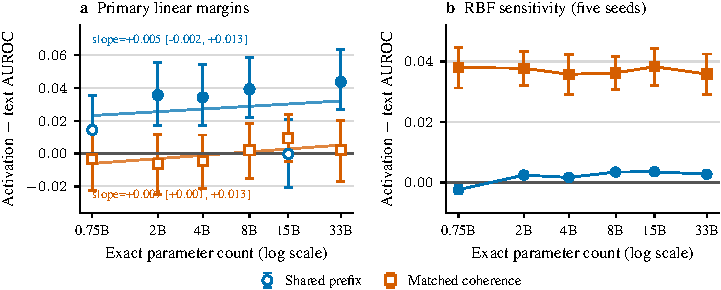
\includegraphics[width=\linewidth]{figures/qwen_scale_ladder.pdf}
  \caption{Within-family Qwen3 scale ladder. \textbf{(a)} Primary linear
  activation-minus-strongest-text margins with 95\% pair-bootstrap intervals
  and fitted slopes. Only the coherence-matched slope interval excludes zero,
  so the prespecified two-control criterion is not met. \textbf{(b)} Post-result
  activation-RBF-minus-contextual-E5 margins, mean $\mathbin{\pm}$ SD over five
  grouped-fold seeds, remain nearly flat with size.}
  \label{fig:qwen-scale}
\end{figure}

\subsection{Steering changes self-report, not refusals}

The prespecified intervention passes its manipulation check: an independent
readout moves monotonically with strength (Spearman $\rho=1.00$), and explicit
evaluation self-reports rise from $0.139$ at coefficient $-2$ to $0.889$ at
$+2$ ($\rho=0.991$). Changing the direction therefore changes the model's own
classification of the setting.

Safety-refusal rates remain between $0.062$ and $0.125$ and trend slightly
opposite to the prediction. With 48 prompts, the test has approximately 80\%
power only against an increase from $0.125$ to about $0.37$; it rules out a
large refusal effect, not smaller policy changes. Steering establishes causal
access to self-report without showing control over broader safety behavior.

\begin{figure}[h]
  \centering
  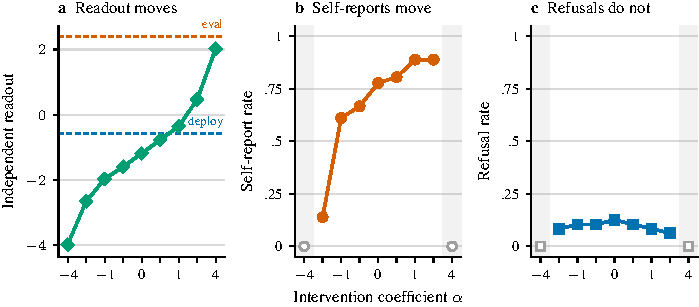
\includegraphics[width=\linewidth]{figures/steering_effects.pdf}
  \caption{Steering moves the independent readout and explicit self-report, but
  not refusal behavior. \textbf{(a)} Independent readout. \textbf{(b)} Evaluation
  self-report rate. \textbf{(c)} Safety-refusal rate. Shaded, hollow endpoints
  violate the frozen output-degeneracy rule and are excluded from trends.}
  \label{fig:steering}
\end{figure}

\FloatBarrier
\section{Discussion}

\subsection{What the direction may represent}

The paired controls narrow, but do not uniquely determine, the content of the
decoded direction. Chance-level separation throughout byte-identical histories
shows that it is not a stable property of the conversation before the final
message. Its sharp onset at that message is consistent with a representation
of evaluation status, but also with benchmark genre, question type, topic
transition, or contextualized speech act. Sparse and frozen contextual
baselines make these alternatives empirically consequential, not merely
philosophical. Conversely, text-level explainability does not mean that
the activation difference is spurious: any representation of the final message
must be caused by that message. It means that the present contrasts do not
identify which abstraction the model uses.

The cross-model, nonlinear, scale, and steering results reinforce this
distinction. All four families create decodable final-turn differences, but
their primary linear margins differ substantially. Nonlinear probes bring all
four close to ceiling within each control without improving cross-control
transfer, while the Qwen3 ladder shows no consistent trend across both
controls. Steering establishes that the Llama direction is causally accessible
and can influence explicit classification of the setting, but not that it
controls a broad behavioral policy. Together, these results support
architecture- and construction-dependent directions rather than a shared,
unitary measure of ``awareness.''

\subsection{Implications for AI evaluation}

For evaluation auditing, raw probe AUROC should be treated as the beginning of
a validity analysis rather than its endpoint. A useful audit should compare
activations with text views matched to what the model has observed, test whether
the signal predates the purported cause, and preserve pairing in both data
splits and uncertainty estimates. Character n-grams and explicit
prefix--ending interactions are important escalation steps because each
overturns a conclusion supported by a weaker comparator. Cross-model
replications should report effect sizes relative to the same baseline, not only
whether each probe exceeds chance. Nonlinear probes should be paired with
capacity-matched text comparators and treated as sensitivity analyses unless
specified before data inspection.

These requirements also change how evaluation-awareness monitors should be
used. A monitor trained on a benchmark-versus-user contrast may be useful for
detecting benchmark-like inputs, even if it does not isolate recognition of
evaluation. That operational use should be stated directly and validated under
the distribution where the monitor will run. Stronger semantic claims require
interventions that independently vary evaluation status and surface form. In
practice, failed controls are informative: the difficulty of creating natural,
indistinguishable endings reveals how tightly evaluation status is entangled
with the way current evaluations are written. A monitor built on an
unvalidated direction would also remain vulnerable if models learned to evade
activation-based monitoring \citep{mcguinness2025chameleons}.

\subsection{Limitations}

Our cross-family evidence is limited to four instruction-tuned open-weight
models in the 8B--12B range, while the within-family audit covers six dense
Qwen3 checkpoints from 0.75B to 32.76B. Six checkpoints from one family do not
establish a universal scaling law or apply directly to frontier proprietary
systems. The primary paired datasets contain 250 examples
per condition and ordinary multi-turn chat, not tool-using agents or long-horizon
tasks. Although the controls remove history-level differences and the
coherence-matched construction reduces topic shift, the final messages are not
counterfactually identical and remain lexically distinguishable. We also do not
independently vary who generated the preceding history, so authorship
invariance remains untested.

Methodologically, the primary estimator is a linear direction of means. The
post-result RBF audit changes the within-control comparison, but it holds the
linearly selected layer fixed and retains the same unresolved semantic
confounds. Its transfer result does not outperform text, so near-ceiling
in-distribution decoding should not be read as construction-invariant. The
observed-silence analysis shows only an absence of detected disclosure, not an
absence of internal reasoning or awareness. Finally, the steering refusal arm
has only 48 prompts and can exclude large effects, not modest behavioral
changes. These limits are why our central claim concerns the validity of current
probe evidence rather than whether any model definitively knows it is being
evaluated.

\section{Conclusion}

We find widespread, temporally localized decodability of evaluation-like versus
deployment-like interactions across four language-model families. Paired
multi-turn conversation controls show that the activation difference is absent
throughout byte-identical histories and appears only after the differing final
turn. Yet its advantage over text depends on the construction and model.
Nonlinear probes improve within-control decoding without improving
cross-control transfer, the Qwen3 ladder shows no consistent trend across both
controls, and steering changes self-report without a detectable safety-refusal
effect.

Probe accuracy therefore does not identify evaluation awareness. It establishes
that a contrast is decodable, not which abstraction the model represents.
Probe-based auditing remains promising, but stronger semantic claims require
controls that separate evaluation status from textual form, competitive text
baselines, generalization across independent constructions, and interventions
tied to behavior. A probe's claimed meaning should be no stronger than the
controls that identify it.

\bibliographystyle{plainnat}
\bibliography{references}

\appendix

\section{Additional experimental details}
\label{app:details}

\subsection{Dataset construction and sampling}

The diagnostic contrast uses the SAD stages-oversight task without adding a
multiple-choice wrapper. Its 200 evaluation examples comprise samples from
three evaluation sources included in SAD; its 200 deployment examples are
WildChat user prompts. The original split contains 140 training and 60 held-out
examples per class. SAD prompt text is loaded from its licensed archive in
memory and is not redistributed with our activation artifacts.

The single-turn transfer grid contains six binary constructions. Two are the
standard and format-controlled pairs from \citet{devbunova2026format}; four
cross two casually rewritten evaluation styles with either rewritten WildChat
requests or same-topic practical requests. Each new cell contains 250 examples.
The initial source mixture is 95 ARC, 58 MMLU, and 97 GSM8K items. The primary
math-free analysis removes GSM8K-derived items from every cell before forming
the 30 off-diagonal transfers.

The retained-history control begins with 250 filtered WildChat conversations of
two to four user turns and replaces only the final user message. The
coherence-matched control jointly constructs a shared everyday prefix and two
same-topic endings. Both sides of each final dataset are model-authored, and
every pair is keyed by a common scenario identifier. The grouped analyses use
that identifier so that alternative endings never cross folds.

The coherence-matched pairs additionally underwent an independent blinded
language-model audit. An isolated \texttt{gpt-5.6-luna} reviewer saw randomized
A/B endings without source identifiers or condition labels and rated coherence,
topic match, and naturalness. Both endings in all 250 pairs were rated coherent,
topic-matched, and at least 3/5 in naturalness; mean ratings were 4.28 for
evaluation endings and 4.22 for deployment endings. The reviewer judged the
evaluation ending more benchmark-like in 198 pairs, the deployment ending in
3, and the two equally benchmark-like in 49. Thus, the audit supports the
intended coherence and topic matching, while confirming that task-form cues
remain.

\subsection{Checkpoint and extraction details}

The replication repositories and frozen revision prefixes are Qwen/Qwen3-8B
at \texttt{b968826d9c46}, google/gemma-3-12b-it at
\texttt{96b6f1eccf38}, and
mistralai/Ministral-3-8B-Instruct-2512-BF16 at
\texttt{f6fae9795746}. Full 40-character revisions, dataset hashes, manifest
hashes, and adapter identities are embedded in each result artifact. Extraction
uses unquantized bfloat16, batch size one, and the model-native chat template.
The prespecified primary readout is the residual-stream state at the token
closing the user turn. For layer selection, the embedding output is indexed as
layer zero.

The scale-ladder revisions are Qwen/Qwen3-0.6B at
\texttt{c1899de289a0}, 1.7B at \texttt{70d244cc86cc}, 4B at
\texttt{1cfa9a720891}, 8B at \texttt{b968826d9c46}, 14B at
\texttt{40c069824f42}, and 32B at \texttt{9216db5781bf}. They are all original
dense Qwen3 checkpoints and are run on the same single A100-SXM4-80GB
environment. Sparse MoE checkpoints, later Qwen generations, and quantized
weights are excluded before execution.

For the replication suite, each user-turn boundary is rendered and processed
as an independent causal prefix. This was frozen after a full-sequence smoke
test exposed suffix-length-dependent bfloat16 differences at otherwise
identical earlier tokens. Rejected smoke caches are isolated from the full-run
artifacts. Each completed model processes all 250 scenarios under both paired
controls, and every pre-final equality check is performed before probe fitting.

\subsection{Probe fitting and inference details}
\label{app:fitting-details}

Repeated-holdout estimates use five paired 70/30 splits. Direct probe--text and
cross-model comparisons use grouped five-fold out-of-fold predictions, with
both endings of each scenario in the same fold and grouped layer selection
nested inside each outer training fold. We report signed AUROC when orientation
matters and separation strength $|\mathrm{AUROC}-0.5|$ for transfer. A
standardized L2-logistic probe and full-pipeline label permutations test
estimator and layer-selection robustness.

The post-result capacity audit fits a standardized RBF-kernel SVM at each outer
fold's primary-selected layer. Scaling, $C\in\{0.1,1,10\}$, and a
dimension-normalized kernel-width grid are selected in pair-grouped inner
folds; no nonlinear layer search is performed. The full grouped analysis is
repeated over fold seeds 0--4. For nonlinear transfer, layer, orientation, and
RBF hyperparameters are selected on the source control only before fitting all
source pairs and scoring the other control.

Text baselines include length, 13 structural features, unigram counts, word
1--2-gram TF--IDF, and character-within-word 3--5-gram TF--IDF. Frozen E5 views
include the ending, full visible conversation, and concatenated prefix and
ending embeddings with their absolute difference and elementwise product. The
capacity-matched comparison applies RBF classifiers to sparse TF--IDF and E5
views, including an exact comparison with the strongest E5 prefix--ending
interaction. Pair-cluster bootstrap intervals use 2,000 draws; paired
approximate randomization swaps prediction vectors within scenarios. The scale
audit uses 5,000 paired draws that resample common scenario IDs across sizes and
refit the OLS slope against $\log_{10}$ exact parameter count.

\section{Complete results}
\label{app:results}

\subsection{Temporal and estimator robustness}

Table~\ref{tab:appendix-estimators} reports the second-estimator check. Both
linear estimators reproduce the final-turn effects and the paired pre-final
nulls. The permutation test reruns layer selection after each label shuffle;
the smallest attainable value with 500 draws is $1/501$.

\begin{table}[h]
  \caption{Repeated-holdout AUROC (mean $\mathbin{\pm}$ standard deviation over
  five paired 70/30 splits). Permutation $p$ corresponds to the
  direction-of-means pipeline.}
  \label{tab:appendix-estimators}
  \centering
  \small
  \begin{tabular}{lccc}
    \toprule
    Contrast/readout & Direction of means & L2 logistic & Permutation $p$ \\
    \midrule
    Diagnostic benchmark/user, final & $0.9918\pm0.0085$ & $0.9933\pm0.0077$ & 0.002 \\
    Retained-history, final & $0.9917\pm0.0033$ & $0.9976\pm0.0017$ & 0.002 \\
    Retained-history, pre-final & $0.4985\pm0.0011$ & $0.5001\pm0.0003$ & 0.990 \\
    Coherence-matched, final & $0.9513\pm0.0115$ & $0.9894\pm0.0081$ & 0.002 \\
    Coherence-matched, pre-final & $0.4990\pm0.0015$ & $0.4992\pm0.0024$ & 0.940 \\
    \bottomrule
  \end{tabular}
\end{table}

The full retained-history trajectory is $0.9917$ at the final turn and $0.4975$,
$0.5003$, and $0.5003$ at one, two, and three user turns before the end. The
corresponding numbers of available pairs are 250, 250, 145, and 61. Thus, the
pre-final null does not depend on choosing only one boundary.

\subsection{Within-family Qwen3 scale ladder}
\label{app:qwen-scale}

\begin{table}[h]
  \caption{Qwen3 scale ladder. Linear entries are primary grouped-OOF
  activation-minus-strongest-text AUROC; nonlinear entries are activation RBF
  minus fixed contextual E5, mean over five fold seeds.}
  \label{tab:qwen-scale}
  \centering
  \scriptsize
  \setlength{\tabcolsep}{3.4pt}
  \begin{tabular}{lrrrr}
    \toprule
      & \multicolumn{2}{c}{Primary linear $\Delta$} &
        \multicolumn{2}{c}{Nonlinear mean $\Delta$} \\
    \cmidrule(lr){2-3}\cmidrule(lr){4-5}
    Exact size & Shared & Coherent & Shared & Coherent \\
    \midrule
    0.75B & $+0.0144$ & $-0.0035$ & $-0.0024$ & $+0.0380$ \\
    2.03B & $+0.0355$ & $-0.0061$ & $+0.0024$ & $+0.0378$ \\
    4.02B & $+0.0341$ & $-0.0046$ & $+0.0017$ & $+0.0358$ \\
    8.19B & $+0.0391$ & $+0.0019$ & $+0.0035$ & $+0.0362$ \\
    14.77B & $-0.0003$ & $+0.0092$ & $+0.0036$ & $+0.0383$ \\
    32.76B & $+0.0436$ & $+0.0019$ & $+0.0027$ & $+0.0358$ \\
    \bottomrule
  \end{tabular}
\end{table}

The primary paired-bootstrap slopes are $+0.0054$
$[-0.0017,+0.0129]$ (retained-history) and $+0.0068$
$[+0.0013,+0.0132]$ (coherence-matched). They fail the frozen criterion because
only one interval excludes zero. For secondary transfer, shared-to-coherent has
slope $-0.0529$ $[-0.0664,-0.0389]$, whereas coherent-to-shared has slope
$-0.0002$ $[-0.0156,+0.0149]$. These six checkpoints test an internal-family
pattern for this pipeline, not a universal scaling law.

\FloatBarrier
\subsection{Cross-model readout sensitivity}
\label{app:readout-sensitivity}

\begin{table}[h]
  \caption{Uniform readout audit using the same paired folds and nested grouped
  layer selection. Entries are probe AUROCs. ``Token'' is the prespecified state
  at the token closing the final user turn. ``Mean (all)'' averages the final
  user turn and permits embedding layer zero; ``Mean ($L\geq1$)'' excludes that
  layer. The unchanged strongest-text AUROCs are 0.9529 (retained-history) and
  0.9447 (coherence-matched).}
  \label{tab:appendix-readout}
  \centering
  \scriptsize
  \setlength{\tabcolsep}{2.8pt}
  \begin{tabular}{lrr@{\qquad}rrr}
    \toprule
      & \multicolumn{2}{c}{Retained-history} & \multicolumn{3}{c}{Coherence-matched} \\
    \cmidrule(lr){2-3}\cmidrule(lr){4-6}
    Model & Token & Mean & Token & Mean (all) & Mean ($L\geq1$) \\
    \midrule
    Llama-3.1-8B & 0.9878 & 0.9916 & 0.9468 & 0.9322 & 0.9325 \\
    Qwen3-8B & 0.9919 & 0.9785 & 0.9450 & 0.9439 & 0.9332 \\
    Gemma-3-12B & 0.9730 & 0.9488 & 0.8590 & 0.9388 & 0.6380 \\
    Ministral-3-8B & 0.9831 & 0.9869 & 0.9279 & 0.8775 & 0.9380 \\
    \bottomrule
  \end{tabular}
\end{table}

Mean pooling is not uniformly better. Under coherence matching, permitting every
layer raises Gemma from 0.8590 to 0.9388 but lowers Ministral from 0.9279 to
0.8775; the direct mean-minus-token changes are $+0.0797$
($[+0.0563,+0.1037]$) and $-0.0504$ ($[-0.0710,-0.0288]$), respectively.
Crucially, Gemma and Qwen select layer zero in all five unrestricted-mean outer
folds (Llama in three; Ministral in one). Layer zero here is the mean of input
token embeddings, not a transformer-computed state. When it is excluded,
Llama, Qwen, and Ministral cluster at 0.9325--0.9380, whereas Gemma falls to
0.6380 and selects layers 4, 4, 48, 7, and 48. The audit therefore does not
support a simple extraction-failure explanation for the primary Gemma result:
the apparent alignment under unrestricted mean pooling is carried by a lexical
embedding average, and the broader finding is architecture-by-readout
sensitivity. We retain the prespecified closing-token readout rather than
selecting a post-result readout for visual alignment.

\subsection{Nonlinear probe sensitivity}
\label{app:nonlinear-probe}

\begin{table}[h]
  \caption{Post-result nonlinear-capacity audit at the prespecified closing-token
  readout (fold seed 0). ``RBF'' holds the primary-selected layer fixed while
  fitting scaling and kernel hyperparameters in pair-grouped inner folds.
  $\Delta$ is activation RBF minus a capacity-matched RBF over the previously
  strongest frozen E5 prefix--ending interaction (0.9953 shared; 0.9566
  coherent).}
  \label{tab:appendix-nonlinear}
  \centering
  \scriptsize
  \setlength{\tabcolsep}{2.7pt}
  \begin{tabular}{lrr@{\qquad}rr}
    \toprule
      & \multicolumn{2}{c}{Retained-history} & \multicolumn{2}{c}{Coherence-matched} \\
    \cmidrule(lr){2-3}\cmidrule(lr){4-5}
    Model & RBF & $\Delta$ E5 & RBF & $\Delta$ E5 \\
    \midrule
    Llama-3.1-8B & 0.9978 & $+0.0025$ & 0.9870 & $\mathbf{+0.0304}$ \\
    Qwen3-8B & 0.9992 & $\mathbf{+0.0039}$ & 0.9879 & $\mathbf{+0.0313}$ \\
    Gemma-3-12B & 0.9899 & $-0.0055$ & 0.9811 & $\mathbf{+0.0245}$ \\
    Ministral-3-8B & 0.9988 & $\mathbf{+0.0034}$ & 0.9871 & $\mathbf{+0.0305}$ \\
    \bottomrule
  \end{tabular}
\end{table}

The nonlinear gain is largest where the primary result was weakest. On matched
coherence, RBF-minus-linear is $+0.1221$ for Gemma
($[+0.0912,+0.1530]$), compared with $+0.0402$ for Llama,
$+0.0428$ for Qwen, and $+0.0592$ for Ministral; all four intervals exclude
zero. Against the stronger E5 RBF, the coherence-matched margins and intervals
are respectively $+0.0304$ $[+0.0149,+0.0461]$, $+0.0313$
$[+0.0164,+0.0465]$, $+0.0245$ $[+0.0100,+0.0388]$, and $+0.0305$
$[+0.0158,+0.0459]$. On the retained-history control, only Qwen and Ministral have positive
intervals; Llama's interval crosses zero and Gemma is numerically below E5 with
an interval that also crosses zero.

Repeating the complete nested analysis over fold seeds 0--4 leaves the
coherence-matched result intact. Mean activation RBF AUROC ranges from
0.9844--0.9897 (SD 0.0015--0.0023), and every model exceeds the fixed E5 RBF in
every seed; mean margins are $+0.0388$, $+0.0390$, $+0.0348$, and $+0.0401$ for
Llama, Qwen, Gemma, and Ministral. Retained-history margins remain stable but
heterogeneous: $+0.0020$, $+0.0035$, $-0.0071$, and $+0.0024$.

\begin{table}[h]
  \caption{Nonlinear cross-control transfer, mean $\mathbin{\pm}$ SD over five
  source-selection fold seeds. Activation RBF layer, orientation, and kernel
  settings are selected on the source only. The nested nonlinear text row
  likewise selects sparse TF--IDF or a frozen E5 view on the source only. The
  final row gives the stronger existing linear character-TF--IDF comparator.}
  \label{tab:appendix-nonlinear-transfer}
  \centering
  \small
  \begin{tabular}{lrr}
    \toprule
    Method/model & Shared $\rightarrow$ coherent & Coherent $\rightarrow$ shared \\
    \midrule
    Llama RBF & $0.772\mathbin{\pm}0.016$ & $0.708\mathbin{\pm}0.005$ \\
    Qwen RBF & $0.806\mathbin{\pm}0.014$ & $0.819\mathbin{\pm}0.013$ \\
    Gemma RBF & $0.715\mathbin{\pm}0.011$ & $0.809\mathbin{\pm}0.000$ \\
    Ministral RBF & $0.717\mathbin{\pm}0.000$ & $0.842\mathbin{\pm}0.006$ \\
    Nonlinear text & $0.827\mathbin{\pm}0.000$ & $0.830\mathbin{\pm}0.030$ \\
    Linear character TF--IDF & 0.866 & 0.849 \\
    \bottomrule
  \end{tabular}
\end{table}

Nonlinear activation transfer is below the text comparator for every model in
the shared-to-coherent direction and does not reliably exceed it in the reverse
direction. The near-ceiling within-control gains therefore do not reveal a
construction-invariant nonlinear signal. Because the audit was motivated by
the observed linear results and holds the linearly chosen layer fixed, it
supports nonlinear decodability rather than a post-hoc replacement of the
primary estimator or a semantic identification claim.

\subsection{Sparse-text comparisons and transfer}

\begin{figure}[h]
  \centering
  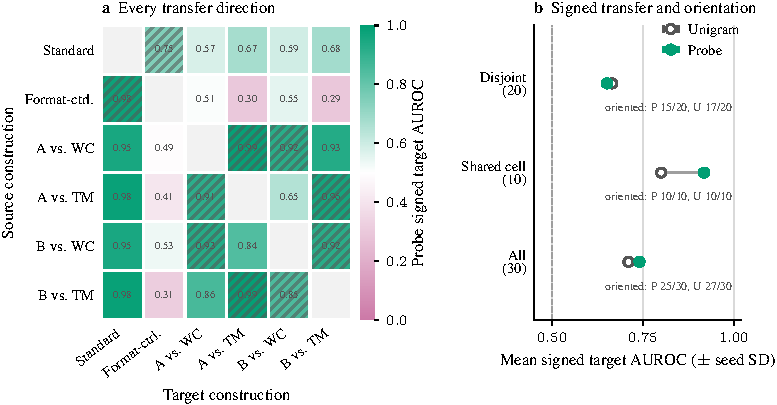
\includegraphics[width=\linewidth]{figures/disjoint_transfer.pdf}
  \caption{Cross-construction transfer against unigram counts on the math-free
  grid. Separation strength is the distance of AUROC from chance.
  \textbf{(a)} Seed-averaged probe-minus-unigram margin for every ordered
  transfer; hatched cells share a constituent dataset cell.
  \textbf{(b)} Mean strength by subset, with the number of transfers in
  parentheses and paired margin (mean $\mathbin{\pm}$ SD over five seeds).}
  \label{fig:transfer}
\end{figure}

\begin{table}[h]
  \caption{Reference-model grouped sparse-text audit. Intervals resample paired
  scenarios; $p$ is one-sided for the prespecified alternative that the probe
  exceeds text.}
  \label{tab:appendix-strong-text}
  \centering
  \small
  \begin{tabularx}{\linewidth}{@{}Yrrrr@{}}
    \toprule
    Analysis & Probe & Text & Difference (95\% interval) & $p$ \\
    \midrule
    Retained-history, within
      & 0.9878 & 0.9529 & $+0.0349$ $[+0.0183,+0.0540]$ & 0.0015 \\
    Coherence-matched, within
      & 0.9468 & 0.9447 & $+0.0021$ $[-0.0134,+0.0168]$ & 0.4378 \\
    Shared $\rightarrow$ coherence
      & 0.8450 & 0.8661 & $-0.0212$ $[-0.0489,+0.0081]$ & 0.8786 \\
    Coherence $\rightarrow$ shared
      & 0.7187 & 0.8485 & $-0.1298$ $[-0.1665,-0.0908]$ & 1.0000 \\
    \bottomrule
  \end{tabularx}
\end{table}

The observed-silence analysis retains 192 coherence-matched pairs; the probe
and unigram AUROCs are $0.9369$ and $0.9354$. The retained-history 512-token
sensitivity run retains 227 pairs and yields $0.9908$ versus $0.9460$. In every
tested cell, the detector finds zero positive awareness disclosures among 250
generated replies; planted-control validation catches all 14 positives with no
false alarms among ten negatives.

For steering, the selected layer is 14. Across nondegenerate coefficients
$-2,-1,-0.5,0,0.5,1,2$, evaluation self-report rates are respectively
$0.139,0.611,0.667,0.778,0.806,0.889,0.889$. Safety-refusal rates over the same
grid are $0.083,0.104,0.104,0.125,0.104,0.083,0.062$. Coefficients $\pm4$ fail
the frozen repetition/degeneracy rule and are excluded from both trends.

\section{Failed and rejected controls}
\label{app:failures}

The experimental sequence contained several probe-blind failures. Reporting
them matters because each failure removes an interpretation that a high AUROC
would otherwise invite.

\paragraph{Single-turn surface gate.}
Length matching succeeds in the four new cells, but format and lexical matching
do not. Five-fold out-of-fold surface AUROCs are:

\begin{table}[h]
  \caption{Surface gate for the four new single-turn contrasts. WC denotes the
  WildChat-derived deployment cell and TM the topic-matched deployment cell.}
  \label{tab:appendix-surface-gate}
  \centering
  \small
  \begin{tabular}{lrrrr}
    \toprule
    Contrast & Character length & Word length & Format & Unigram \\
    \midrule
    Eval A vs. WC & 0.4726 & 0.4932 & 0.6627 & 0.9319 \\
    Eval A vs. TM & 0.4764 & 0.4673 & 0.8326 & 0.9783 \\
    Eval B vs. WC & 0.4923 & 0.5222 & 0.7818 & 0.9056 \\
    Eval B vs. TM & 0.4964 & 0.4954 & 0.7435 & 0.9135 \\
    \bottomrule
  \end{tabular}
\end{table}

\paragraph{Leaking multi-turn construction.}
The first written ``disguised evaluation'' cell obtains final-boundary probe
AUROC $0.9846$, but its probe is already at $0.9492$ after the first user turn,
before the benchmark question appears. Its synthetic histories therefore leak
the label and cannot support temporal localization. We retain the result only
as the failure that motivated the retained-history recombination.
Figure~\ref{fig:leak} contrasts the two constructions.

\begin{figure}[ht]
  \centering
  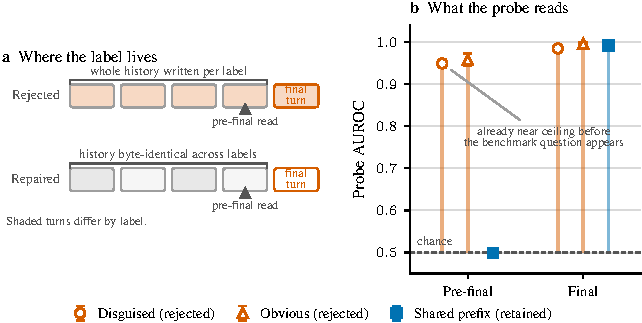
\includegraphics[width=\linewidth]{figures/failed_temporal_control.pdf}
  \caption{The rejected leaking construction against the repaired control.
  \textbf{(a)} In the written cells the whole history is authored per label, so
  the class is present before the final turn; the retained-history recombination
  makes the history byte-identical across labels. \textbf{(b)} Reference-model
  probe AUROC at each read point (mean $\mathbin{\pm}$ standard deviation over
  five train/test splits). Both rejected cells are already near ceiling at the
  pre-final read, which is what disqualifies them; only the retained-history
  control sits at chance there.}
  \label{fig:leak}
\end{figure}

\paragraph{Rejected coherence attempt.}
An initial attempt appended unrelated benchmark items to frozen deployment
histories. Although activations were extracted, manual review found many endings
incoherent with their histories. The dataset was rejected before being used as
a successful control; the reported coherence-matched results come from the
jointly constructed replacement.

\paragraph{Authorship-factorial pilot.}
A prespecified pilot attempted to vary evaluation status independently of the
model that generated the preceding history. All 150 histories terminated, but
the combined blinded model and frozen human coherence gate retained only 36 of
50 scenarios, below its 40-scenario activation threshold. No activations were
extracted or inspected. Consequently, this paper makes no claim that the
direction is invariant to history authorship.

\end{document}
